	\chapter*{Abstract}

	\textit{This work introduces the students to some properties of cosmic radiation at ground level, in particular, its hard or muon component. First, it shows how to use a wave-guide to determine the working point of two scintillators associated with photomultiplier detectors, obtaining the values V$_\text{threshold}$ ​​= $-$200 mV and HV = 1900 V or HV = 2200 V. It also shows how to determine the value of the time window of the measurement system which has a width of 50 ns.}

	\textit{Making measurements in these working conditions, it is demonstrated that cosmic radiation is statistical in nature and conforms specifically to a Normal or Gaussian distribution. On the other hand, it is possible to separate the contributions of the hard and soft components of the cosmic radiation at ground-level, by making the total flux pass through increasing values of the thickness of lead and aluminium layers of material. Under these conditions, a value ​​of 51 $\pm$ 5 m$^{-2}$s$^{-1}$ is obtained for the hard component of the flux, and 31 $\pm$ 10 m$^{-2}$s$^{-1}$ for the soft component.}

	\textit{Regarding the reliability of the measurements, the effect of the distance between the two scintillators is also evaluated, by calculating the geometric efficiency experimentally and then contrasting the resulting value with the one obtained from a calculation based on a Monte Carlo simulation. These results imply that the system efficiency decreases in proportion to the inverse square of the distance between the detectors.}

	\bfi[H]
		\bc
			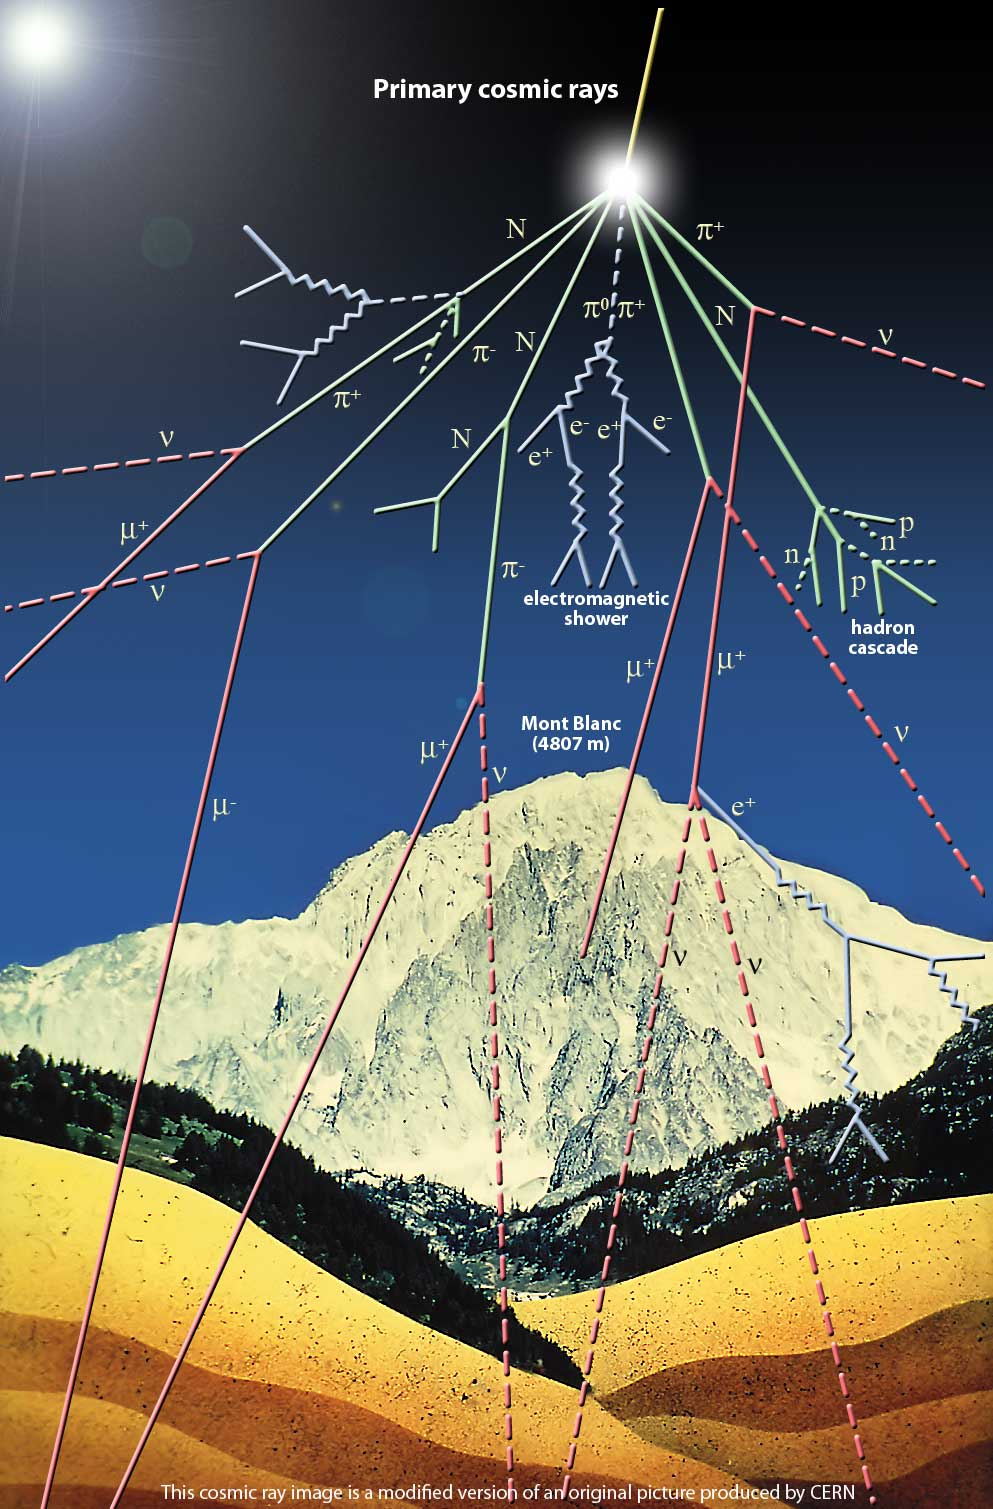
\includegraphics[width=.9\textwidth]{img/cosmic-rays.jpg}\\[12pt]
			\caption
				[Cosmic rays are immensely high-energy radiation, mainly originating outside the Solar System.]
				{Cosmic rays are immensely high-energy radiation, mainly originating outside the Solar System. They may produce showers of secondary particles that penetrate and impact the Earth's atmosphere and sometimes even reach the surface.	(Courtesy: CERN)}
		\ec
		\label{fig:cosmicrays}
	\efi

	\cleardoublepage

